\documentclass[12pt]{article}

\usepackage{graphicx}
\usepackage{hyperref}
\usepackage{amssymb}
\usepackage{amsmath}
\usepackage{amsthm}
\usepackage{algorithm}
\usepackage{algorithmic}
\usepackage{graphicx}  
\usepackage{caption}  
\usepackage{subcaption}
\usepackage{float}
\usepackage{titlesec}
\usepackage{titletoc}
\usepackage{tocloft} % For modifying the TOC spacing
\usepackage{xcolor}  % For coloring section titles
\usepackage[a4paper, total={7.25in, 9.5in}]{geometry}
\usepackage{placeins}

\newcommand{\scale}{0.4} 
\newcommand{\scaletwo}{0.35}
\newcommand{\correlation}{0.25}
\newcommand{\parameter}{0.35}

\usepackage{anyfontsize}
\fontsize{11pt}{13pt}\selectfont

\usepackage[style = authoryear, backend = biber]{biblatex}
\addbibresource{references.bib}

\title{Model and Variable Comparison}
\author{Nick Bossi}
\date{February 2025}

\begin{document}
	
\begin{titlepage}
	\begin{center}
		\vspace*{2cm}
		{\LARGE\bfseries Model and Variable Comparison\par}
		\vspace{1cm}
		{\large\bfseries Nick Bossi\par}
		\vspace{0.5cm}
		{\large\bfseries February 2025\par}
		\vspace{2cm}
		
		\tableofcontents
	\end{center}
\end{titlepage}
	
\section{Introduction}
16 Models were fitted to the rat data, namely:
\begin{enumerate}
	\item Random Response (rr)
	\item Contextual Random Response (crr)
	\item Win-Stay Shift-Lose (wsls)
	\item Rescorla-Wagner (rw)
	\item Contextual Rescorla-Wagner (crw)
	\item Choice-Kernel (ck)
	\item Contextual Rescorla-Wagner and Choice-Kernel (crwck)
	\item Contextual Rescorla-Wagner and Choice-Kernel Shared Alpha (crwcksa)
	\item Contextual Rescorla-Wagner and Choice-Kernel No Beta (crwcknb)
	\item Contextual Rescorla-Wagner and Choice-Kernel All (crwck\_all)
	\item Contextual Rescorla-Wagner and Choice-Kernel Pre-Fitted (crwck\_pre)
	\item Contextual Rescorla-Wagner and Choice-Kernel Initialised (crwck\_init)
	\item Contextual Rescorla-Wagner and Choice-Kernel Plus (crwck\_plus).
	\item Contextual Rescorla-Wagner and Choice-Kernel Shared Alpha Plus (crwcksa\_plus)
	\item Contextual Rescorla-Wagner and Choice-Kernel Plus Pre-Fitted (crwck\_plus\_pre)
	\item Contextual Rescorla-Wagner and Choice-Kernel Plus Initialised (crwck\_plus\_init)
\end{enumerate}

\section{Methodology Section}
\subsection{Experiment}
The experiment investigates learning and attention mechanisms in rats. At each trial, two modes of stimuli are presented to the rats, namely a visual and auditory stimulus. During each session (collection of trials grouped by some common property), one of the modes was chosen to be the ``relevant mode", meaning that reward responses were only as a result of which stimulus was presented in that mode. Namely, each rat was presented with one of two visual and auditory stimuli at each trial. If, for instance, in a given session the visual stimulus was the relevant mode, the two visual stimuli (Viusal1 or Visual2) the rat is exposed to would correspond to either a NOGO or GO response as being rewarded. ie: if Visual1 was presented to the rat and the rat did not run on the treadmill, they would be rewarded. Similarly, if Visual2 was presented to the rat and the rat did run on the treadmill, they would be rewarded. In all other scenarios the rat would not receive a reward. The two levels of stimuli of the non-relevant mode (in this example Auditory) would still be presented to each rat at each trial, but would have no consequence on rewards received, and were chosen randomly with equal probability (50-50).
\\\\
For a given relevant modality, there are two ``difficulty levels". The easy level corresponds to a pair of stimulus which are more obviously distinct from one another than the hard level. For example, if the relevant modality is auditory, then for an easy session the two auditory stimuli might be two pitches (sinusoidal sound waves) whose frequencies are greatly different (for example 4.7kHz vs 8.2kHz) whilst for a hard/difficult session the frequencies would be closer together (for example 4.7kHz and 5.2kHz), making it harder to distinguish between the two stimuli of the relevant modality.\\\\
The experiment seeks to investigate if more intense focus during a learning task of one relevant modality affects the subsequent learning task when the relevant modality is shifted (referred to as an Extra-Dimensional Shift (EDS) session). For example, will a rat who was exposed to difficult to distinguish stimuli when the relevant mode is auditory, subsequently learn differently when the relevant mode is visual, as compared to a rat who was exposed to easy to distinguish stimuli when the relevant mode was auditory.
\\\\
Multiple models were fitted to the EDS sessions on a per-rat basis, and the fitted parameters were compared between those individuals who had previously been exposed to an Easy to distinguish stimulus versus those who had been exposed to a Hard to distinguish stimulus. 

\subsection{Fitting Procedures}
Maximum likelihood techniques were used to fit the parameters of each model.
Certain models (namely the Random Response, Contextual Random Response and Win-Stay Lose-Shift models) used analytic techniques in order to find the parameters which maximised the likelihood of the data under the model, as the derivatives of the log-likelihood could be found and solved for in closed form. For the more complex, sequentially defined models, numerical techniques were used. For each model, parameter initialisation ranges were chosen and the scipy.optimize package (\cite{2020SciPy-NMeth}) was used to maximise the likelihood, iterating over all initialisation points to ensure the global minumum was achieved.

\subsection{Model Selection}
Bayesian Information Criterion values were used to judge which model had the best fit. 

\section{Models}
At a given time-point $t$, we describe the action $a_t$, stimulus $s_t$ and reward $r_t$ by:
\begin{align}
		&a_t = \begin{cases}
		0  \qquad  \text{if action is NOGO}\\
		1  \qquad  \text{if action is GO} \\
	\end{cases}\\
		&s_t = \begin{cases}
		0  \qquad  \text{if stimulus is NOGO}\\
		1  \qquad  \text{if stimulus is GO} \\
	\end{cases}\\
		&r_t = \begin{cases}
		1  \qquad  \text{if (action and stimulus is NOGO) or (action and stimulus is GO)}\\
		0  \qquad  \text{otherwise} \\
	\end{cases}
\end{align}



\subsection{Random Response (rr)}
The Random Response Model is a simple model for which the probability of the agent taking a certain action is fixed for each trial, namely:

\begin{align}
	p(a_t) = \begin{cases}
		b \qquad &a_t = \text{NOGO}\\
		1- b \qquad &a_t = \text{GO}
	\end{cases}
\end{align}
The fitted parameters are $\{b\}$.



\subsection{Contextual Random Response (crr)}
The Contextual Random Response Model uses a separate Random Response Model for each stimulus, namely:
\begin{align}
	p(a_t) = \begin{cases}
		b_{s_t} \qquad &a_t = \text{NOGO}\\
		1- b_{s_t} \qquad &a_t = \text{GO}
	\end{cases}
\end{align}
The fitted parameters are $\{b_0, b_1\}$ relating to the two possible stimuli received.

\subsection{Win-Stay, Lose-Shift (wsls)}
The Win-Stay, Lose-Shift Model uses the reward to determine whether an action will be repeated or not, with some randomness.
\begin{align}
	p(a_t) = \begin{cases}
		1 - \epsilon \qquad &\text{if } a_{t-1} = a_t \text{ and } r_{t-1} = 1\\
		\epsilon \qquad &\text{otherwise} 
	\end{cases}
\end{align}
The fitted parameters are $\{\epsilon\}$.

\subsection{Rescorla-Wagner (rw)}
The Rescorla-Wagner Model uses Q-values which keep track of the relative value associated with each action. It has a learning-rate parameter $\alpha$ and randomness parameter $\beta$, with the density being:
\begin{align}
	p(a_t) &= \frac{\text{exp}\left(\beta \times Q_{a_t}\right)}{\sum_{j=0}^1 \text{exp}\left(\beta \times Q_j\right)}
\end{align}
With the Q-values being updated as follows:
\begin{align}
	Q_{a_t} = Q_{a_t} + \alpha \left(r_t - Q_{a_t}\right) 
\end{align}
and Q-values initialised equally meaning there is no prior preference,ie : $Q_{initial} = (0,0)$.\\\\
The fitted parameters are $\{\alpha, \beta\}$.

\subsection{Contextual Rescorla-Wagner (crw)}
The Contextual Rescorla-Wagner keeps track of separate Q-values depending on the stimulus experienced at time $t$. The fitted parameters are shared between stimuli.\\\\
Thus, for an agent experiencing stimuli $s_t$, the resulting density is:
\begin{align}
	p(a_t) &= \frac{\text{exp}\left(\beta \times Q^{s_t}_{a_t}\right)}{\sum_{j=0}^1 \text{exp}\left(\beta \times Q^{s_t}_j\right)}
\end{align}
With the different Q-values being updated identically to that of the Rescorla-Wagner Model:
\begin{align}
	Q^{s_t}_{a_t} = Q^{s_t}_{a_t} + \alpha \left(r_t - Q^{s_t}_{a_t}\right) 
\end{align}
The fitted parameters are $\{\alpha, \beta\}$.
\subsection{Choice-Kernel (ck)}
The Choice-Kernel Model similarly stores values associated with each action, but uses previous actions taken instead of the rewards received to update these values.
\begin{align}
	p(a_t) &= \frac{\text{exp}\left(\beta \times CK_{a_t}\right)}{\sum_{j=0}^1 \text{exp}\left(\beta \times CK_j\right)}
\end{align}
With the Choice-Kernel values being updated as follows:
\begin{align}
	CK_0 = CK_0 + \alpha(c_t - CK_0)\\
	CK_1 = CK_1 + \alpha(c_t - CK_1)
\end{align}
where $c_t = 1$ if the action taken at time $t$ is the same as the action being updated.
\\\\
Both Q and CK-values were initialised to zero.
\\\\
The fitted parameters are $\{\alpha, \beta\}$.

\subsection{Contextual Rescorla-Wagner and Choice-Kernel (crwck)}
The Contextual Rescorla-Wagner and Choice-Kernel Model combines the Rescoral-Wagner and Choice-Kernel Models while additionally keeping track of separate Q and CK-values for each stimulus.\\\\
Thus, for an agent experiencing stimuli $s_t$, the resulting density is:
\begin{align}
	p(a_t) &= \frac{\text{exp}\left(\beta \times \left(Q^{s_t}_{a_t} + CK^{s_t}_{a_t}\right)\right)}{\sum_{j=0}^1 \text{exp}\left(\beta \times \left( Q^{s_t}_{j} +  CK^{s_t}_{j}\right)\right)}
\end{align}
With the different Q and CK-values being updated as before.\\\\
Again, both Q and CK-values were initialised to zero.\\\\
The fitted parameters are $\{\alpha_{rw}, \alpha_{ck}, \beta\}$.

\subsection{Contextual Rescorla-Wagner and Choice-Kernel Shared Alpha (crwcksa)}
The Contextual Rescorla-Wagner and Choice-Kernel Shared Alpha is identical to the crwck model except it has a single learning rate parameter that is used to update both the Q and CK-values.
\\\\
The fitted parameters are $\{\alpha, \beta\}$.

\subsection{Contextual Rescorla-Wagner and Choice-Kernel No Beta (crwcknb)}
The Contextual Rescorla-Wagner and Choice-Kernel No Beta Model is identical to the Contextual Rescorla-Wagner and Choice-Kernel Model however with the $\beta$ parameter removed.\\\\
The fitted parameters are thus $\{\alpha_{rw}, \alpha_{ck}\}$.

\subsection{Contextual Rescorla-Wagner and Choice-Kernel All (crwck\_all)}
The Contextual Rescorla-Wagner and Choice-Kernel All model is the same as the crwck model except that it stores four pairs of Q-values associated with each combination of both the visual and auditory stimulus rather than only storing Q-values associated with the relevant stimulus.
\\\\
Q and CK-values were initialised to zero.
\\\\
The fitted parameters are $\{\alpha_{rw}, \alpha_{ck}, \beta\}$.

\subsection{Contextual Rescorla-Wagner and Choice-Kernel Pre-Fitted (crwck\_pre)}
The Contextual Rescorla-Wagner and Choice-Kernel Pre-Fitted model is identical to the crwck\_all model however Q and CK-values were no longer initialised to zero. Instead, the model is fitted to the previous four sessions (pre-modality shift) and the final Q and CK-values from the previously fitted sessions are used as the intialised Q and CK-values for the final fitting.
\\\\
The fitted parameters are $\{\alpha, \beta_{rw}, \beta_{ck}\}$.

\subsection{Contextual Rescorla-Wagner and Choice-Kernel Initialised (crwck\_init)}
The Contextual Rescorla-Wagner and Choice-Kernel Initialised model combines the crwck and crwck\_pre models in the sense that four pairs of Q and CK-values are initially fitted for the four pre-EDS sessions in the crwck\_pre model, but then only two Q and CK-value pairs of used for the actual EDS sessions. The two pairs are calculated from the old pairs by averaging over the non-relevant modalities values. For example, let $\{Q00, Q01, Q10 \text{ and } Q11\}$ relate to the four pairs of Q-values, with the first number indicating the visual stimulus and the second indicating the auditory stimulus. If the relevant modality is visual, then our new pairs of Q-values would be calculated as:
\begin{align}
	Q0 = \frac{Q00 + Q01}{2}\\
	Q1 = \frac{Q10 + Q11}{2}
\end{align}
where all operations are done component-wise for the pairs.
\\\\
The fitted parameters are $\{\alpha, \beta_{rw}, \beta_{ck}\}$.

\subsection{Contextual Rescorla-Wagner and Choice-Kernel Plus (crwck\_plus)}
The Contextual Rescorla-Wagner and Choice-Kernel Plus Model is identical to the crwck model except that it has separate $\beta$ coefficients for the Q and CK-values.
\begin{align}
	p(a_t) &= \frac{\text{exp}\left(\beta_{rw} \times Q^{s_t}_{a_t} + \beta_{ck} \times CK^{s_t}_{a_t}\right)}{\sum_{j=0}^1 \text{exp}\left(\beta_{rw} \times Q^{s_t}_{j} + \beta_{ck} \times CK^{s_t}_{j}\right)}
\end{align}
The fitted parameters are$\{\alpha_{rw}, \alpha_{ck}, \beta_{rw}, \beta_{ck}\}$.


\subsection{Contextual Rescorla-Wagner and Choice-Kernel Shared Alpha Plus (crwcksa\_plus)}
The Contextual Rescorla-Wagner and Choice-Kernel Plus No Alpha Model is identical to the crwck\_plus model except that it has single learning rate $\alpha$ that is used to update both the Q and Ck-values.
\\\\
The fitted parameters are$\{\alpha, \beta_{rw}, \beta_{ck}\}$.

\subsection{Contextual Rescorla-Wagner and Choice-Kernel Plus Pre-Fitted (crwck\_plus\_pre)}
The Contextual Rescorla-Wagner and Choice-Kernel Plus Pre-Fitted model is similar to the crwck\_plus model but like the crwck\_pre model now uses four pairs of Q and CK-values as well as using pre-fitted Q and CK initial values.
\\\\
The fitted parameters are $\{\alpha_{rw},\alpha_{ck}, \beta_{rw}, \beta_{ck}\}$.
 
 \subsection{Contextual Rescorla-Wagner and Choice-Kernel Plus Initialised (crwck\_plus\_init)}
 The Contextual Rescorla-Wagner and Choice-Kernel Plus Initialised model combines the crwck\_plus and crwck\_plus\_pre models in the same way in which the crwck\_init model combines the crwck and crwck\_pre models.\\\\
 The fitted parameters are $\{\alpha, \beta_{rw}, \beta_{ck}\}$.
\newpage

\section{Model Selection}
A parameter search was conducted for each model, with parameters being chosen which maximized the likelihood of seeing the data under a given model. Once optimal parameters were found for each model, the resultant models' likelihoods and Bayesian Information Criterions (BIC) were compared to determine which model had the best overall fit.

\begin{figure}[h]  % [h] places the figure here
	\centering
	\includegraphics[width=1\textwidth]{D:/Documents/Work/Helsinki_Internship/Code/perceptual_attention_learning/reinforcement_learning/plots/LL/negLL_BIC_plot.png}  % Change 'image.png' to the name of your image file
	\caption{Line graph comparing the negative log-likelihood and BICs of the 14 fitted models, ordered in ascending order of BIC values.}
	\label{fig:internalenvironment}
\end{figure} 

The lowest BIC values correspond to the best fitting models, and consequently the crwcka\_plus model was chosen to be the best fitting model.

\newpage
\section{Parameter Comparison}
 The fitted variables of each rat were compared between the Easy and Hard groups for each model. Lines between points indicate the same rats being compared between the Easy and Hard learning tasks.
 \\\\
 Correlation matrices were also plotted for some of the more complex models.

\subsection{Random Response (rr) Parameter Comparison}


\begin{figure}[h]  % [h] places the figure here
	\centering
	\includegraphics[scale = \parameter]{D:/Documents/Work/Helsinki_Internship/Code/perceptual_attention_learning/reinforcement_learning/plots/param_comparison/rr_param_comparison.png}  % Change 'image.png' to the name of your image file
	\caption{Barchart comparing the optimal parameters for the Random Response model.}
	\label{fig:rr_model_parameters}
\end{figure} 
\clearpage
\newpage
\subsection{Contextual Random Response (crr) Parameter Comparison}


\begin{figure}[h]  % [h] places the figure here
	\centering
	\includegraphics[scale = \parameter]{D:/Documents/Work/Helsinki_Internship/Code/perceptual_attention_learning/reinforcement_learning/plots/param_comparison/crr_param_comparison.png}  % Change 'image.png' to the name of your image file
	\caption{Barchart comparing the optimal parameters for the Contextual Random Response model.}
	\label{fig:crr_model_parameters}
\end{figure} 
\newpage
\clearpage
\subsection{Win-Stay, Lose-Shift (wsls) Parameter Comparison}

\begin{figure}[h]  % [h] places the figure here
	\centering
	\includegraphics[scale = \parameter]{D:/Documents/Work/Helsinki_Internship/Code/perceptual_attention_learning/reinforcement_learning/plots/param_comparison/wsls_param_comparison.png}  % Change 'image.png' to the name of your image file
	\caption{Barchart comparing the optimal parameters for the Win-Stay, Lose-Shift model.}
	\label{fig:wsls_model_parmeters}
\end{figure} 
\clearpage
\newpage

\subsection{Rescorla-Wagner (rw) Parameter Comparison}

\begin{figure}[h]  % [h] places the figure here
	\centering
	\includegraphics[scale = \parameter]{D:/Documents/Work/Helsinki_Internship/Code/perceptual_attention_learning/reinforcement_learning/plots/param_comparison/rw_param_comparison.png}  % Change 'image.png' to the name of your image file
	\caption{Barchart comparing the optimal parameters for the Rescorla-Wagner model.}
	\label{fig:rw_model_parmeters}
\end{figure}
\clearpage
\newpage
\subsection{Contextual Rescorla-Wagner (crw) Parameter Comparison}

\begin{figure}[h]  % [h] places the figure here
	\centering
	\includegraphics[scale = \parameter]{D:/Documents/Work/Helsinki_Internship/Code/perceptual_attention_learning/reinforcement_learning/plots/param_comparison/crw_param_comparison.png}  % Change 'image.png' to the name of your image file
	\caption{Barchart comparing the optimal parameters for the Contextual Rescorla-Wagner model.}
	\label{fig:crw_model_parmeters}
\end{figure}  

\clearpage
\newpage
\subsection{Choice-Kernel (ck) Parameter Comparison}

\begin{figure}[h]  % [h] places the figure here
	\centering
	\includegraphics[scale = \parameter]{D:/Documents/Work/Helsinki_Internship/Code/perceptual_attention_learning/reinforcement_learning/plots/param_comparison/ck_param_comparison.png}  % Change 'image.png' to the name of your image file
	\caption{Barchart comparing the optimal parameters for the Choice-Kernel model.}
	\label{fig:ck_model_parmeters}
\end{figure} 
\clearpage
\newpage
\subsection{Contextual Rescorla-Wagner Choice-Kernel (crwck) Parameter Comparison}
\begin{figure}[h]  % [h] places the figure here
	\centering
	\includegraphics[scale = \parameter]{D:/Documents/Work/Helsinki_Internship/Code/perceptual_attention_learning/reinforcement_learning/plots/param_comparison/crwck_param_comparison.png}  % Change 'image.png' to the name of your image file
	\caption{Barchart comparing the optimal parameters for the Contextual Rescorla-Wagner Choice-Kernel model.}
	\label{fig:crwck_model_parmeters}
\end{figure} 

\subsubsection{Contextual Rescorla-Wagner Choice-Kernel (crwck) Parameter Correlation Matrix}

\begin{figure}[h]  % [h] places the figure here
	\centering
	\includegraphics[scale = \correlation]{D:/Documents/Work/Helsinki_Internship/Code/perceptual_attention_learning/reinforcement_learning/plots/correlation/correlation_matrices/crwck_correlation.png}  % Change 'image.png' to the name of your image file
	\caption{Correlation matrix of the optimal parameters for the Contextual Rescorla-Wagner Choice-Kernel model.}
	\label{fig:crwck_correlation_matrix}
\end{figure} 
\clearpage
\newpage
\subsection{Contextual Rescorla-Wagner Choice-Kernel (crwcknb) No Beta Parameter Comparison}

\begin{figure}[h]  % [h] places the figure here
	\centering
	\includegraphics[scale = \parameter]{D:/Documents/Work/Helsinki_Internship/Code/perceptual_attention_learning/reinforcement_learning/plots/param_comparison/crwcknb_param_comparison.png}  % Change 'image.png' to the name of your image file
	\caption{Barchart comparing the optimal parameters for the Contextual Rescorla-Wagner Choice-Kernel No Beta model.}
	\label{fig:crwcknb_model_parmeters}
\end{figure} 

\clearpage

\subsection{Contextual Rescorla-Wagner Choice-Kernel All (crwck\_all) Parameter Comparison}

\begin{figure}[h]  % [h] places the figure here
	\centering
	\includegraphics[scale = \parameter]{D:/Documents/Work/Helsinki_Internship/Code/perceptual_attention_learning/reinforcement_learning/plots/param_comparison/crwck_all_param_comparison.png}  % Change 'image.png' to the name of your image file
	\caption{Barchart comparing the optimal parameters for the Contextual Rescorla-Wagner Choice-Kernel All model.}
	\label{fig:crwck_all_model_parmeters}
\end{figure} 
\newpage

\subsection{Contextual Rescorla-Wagner Choice-Kernel Shared Alpha (crwcksa) Parameter Comparison}

\begin{figure}[h]  % [h] places the figure here
	\centering
	\includegraphics[scale = \parameter]{D:/Documents/Work/Helsinki_Internship/Code/perceptual_attention_learning/reinforcement_learning/plots/param_comparison/crwcksa_param_comparison.png}  % Change 'image.png' to the name of your image file
	\caption{Barchart comparing the optimal parameters for the Contextual Rescorla-Wagner Choice-Kernel Shared Alpha model.}
	\label{fig:crwcksa_model_parmeters}
\end{figure} 

\subsubsection{Contextual Rescorla-Wagner Choice-Kernel Shared Alpha (crwcksa) Parameter Correlation Matrix}

\begin{figure}[h]  % [h] places the figure here
	\centering
	\includegraphics[scale = \correlation]{D:/Documents/Work/Helsinki_Internship/Code/perceptual_attention_learning/reinforcement_learning/plots/correlation/correlation_matrices/crwcksa_correlation.png}  % Change 'image.png' to the name of your image file
	\caption{Correlation matrix of the optimal parameters for the Contextual Rescorla-Wagner Choice-Kernel Shared Alpha model.}
	\label{fig:crwcksa_correlation_matrix}
\end{figure} 
\newpage


\subsection{Contextual Rescorla-Wagner Choice-Kernel Pre-Fitted (crwck\_pre) Parameter Comparison}

\begin{figure}[h]  % [h] places the figure here
	\centering
	\includegraphics[scale = \parameter]{D:/Documents/Work/Helsinki_Internship/Code/perceptual_attention_learning/reinforcement_learning/plots/param_comparison/crwck_pre_param_comparison.png}  % Change 'image.png' to the name of your image file
	\caption{Barchart comparing the optimal parameters for the Contextual Rescorla-Wagner Choice-Kernel Pre-Fitted model.}
	\label{fig:crwck_pre_model_parmeters}
\end{figure} 

\subsubsection{Contextual Rescorla-Wagner Choice-Kernel Pre-Fitted (crwck\_pre) Parameter Correlation Matrix}

\begin{figure}[h]  % [h] places the figure here
	\centering
	\includegraphics[scale = \correlation]{D:/Documents/Work/Helsinki_Internship/Code/perceptual_attention_learning/reinforcement_learning/plots/correlation/correlation_matrices/crwck_pre_correlation.png}  % Change 'image.png' to the name of your image file
	\caption{Correlation matrix of the optimal parameters for the Contextual Rescorla-Wagner Choice-Kernel Pre-Fitted model.}
	\label{fig:crwck_pre_correlation_matrix}
\end{figure} 
\newpage

\subsection{Contextual Rescorla-Wagner Choice-Kernel Initialised (crwck\_init) Parameter Comparison}

\begin{figure}[h]  % [h] places the figure here
	\centering
	\includegraphics[scale = \parameter]{D:/Documents/Work/Helsinki_Internship/Code/perceptual_attention_learning/reinforcement_learning/plots/param_comparison/crwck_init_param_comparison.png}  % Change 'image.png' to the name of your image file
	\caption{Barchart comparing the optimal parameters for the Contextual Rescorla-Wagner Choice-Kernel Initialised model.}
	\label{fig:crwck_init_model_parmeters}
\end{figure}
\newpage

\subsection{Contextual Rescorla-Wagner Choice-Kernel Plus Parameter Comparison}

\begin{figure}[h]  % [h] places the figure here
	\centering
	\includegraphics[scale=\parameter]{D:/Documents/Work/Helsinki_Internship/Code/perceptual_attention_learning/reinforcement_learning/plots/param_comparison/crwck_plus_param_comparison.png}  % Change 'image.png' to the name of your image file
	\caption{Barchart comparing the optimal parameters for the Contextual Rescorla-Wagner Choice-Kernel Plus model.}
	\label{fig:crwck_plus_model_parmeters}
\end{figure} 

\subsubsection{Contextual Rescorla-Wagner Choice-Kernel Plus Parameter Correlation Matrix}

\begin{figure}[h]  % [h] places the figure here
	\centering
	\includegraphics[scale = \correlation]{D:/Documents/Work/Helsinki_Internship/Code/perceptual_attention_learning/reinforcement_learning/plots/correlation/correlation_matrices/crwck_plus_correlation.png}  % Change 'image.png' to the name of your image file
	\caption{Correlation matrix of the optimal parameters for the Contextual Rescorla-Wagner Choice-Kernel Plus model.}
	\label{fig:crwck_plus_correlation_matrix}
\end{figure} 
\newpage

\subsection{Contextual Rescorla-Wagner Choice-Kernel Shared Alpha Plus Parameter Comparison}

\begin{figure}[h]  % [h] places the figure here
	\centering
	\includegraphics[scale=\parameter]{D:/Documents/Work/Helsinki_Internship/Code/perceptual_attention_learning/reinforcement_learning/plots/param_comparison/crwcksa_plus_param_comparison.png}  % Change 'image.png' to the name of your image file
	\caption{Barchart comparing the optimal parameters for the Contextual Rescorla-Wagner Choice-Kernel Shared Alpha Plus model.}
	\label{fig:crwcksa_plus_model_parmeters}
\end{figure} 

\subsubsection{Contextual Rescorla-Wagner Choice-Kernel Shared Alpha Plus Parameter Correlation Matrix}
\begin{figure}[h]  % [h] places the figure here
	\centering
	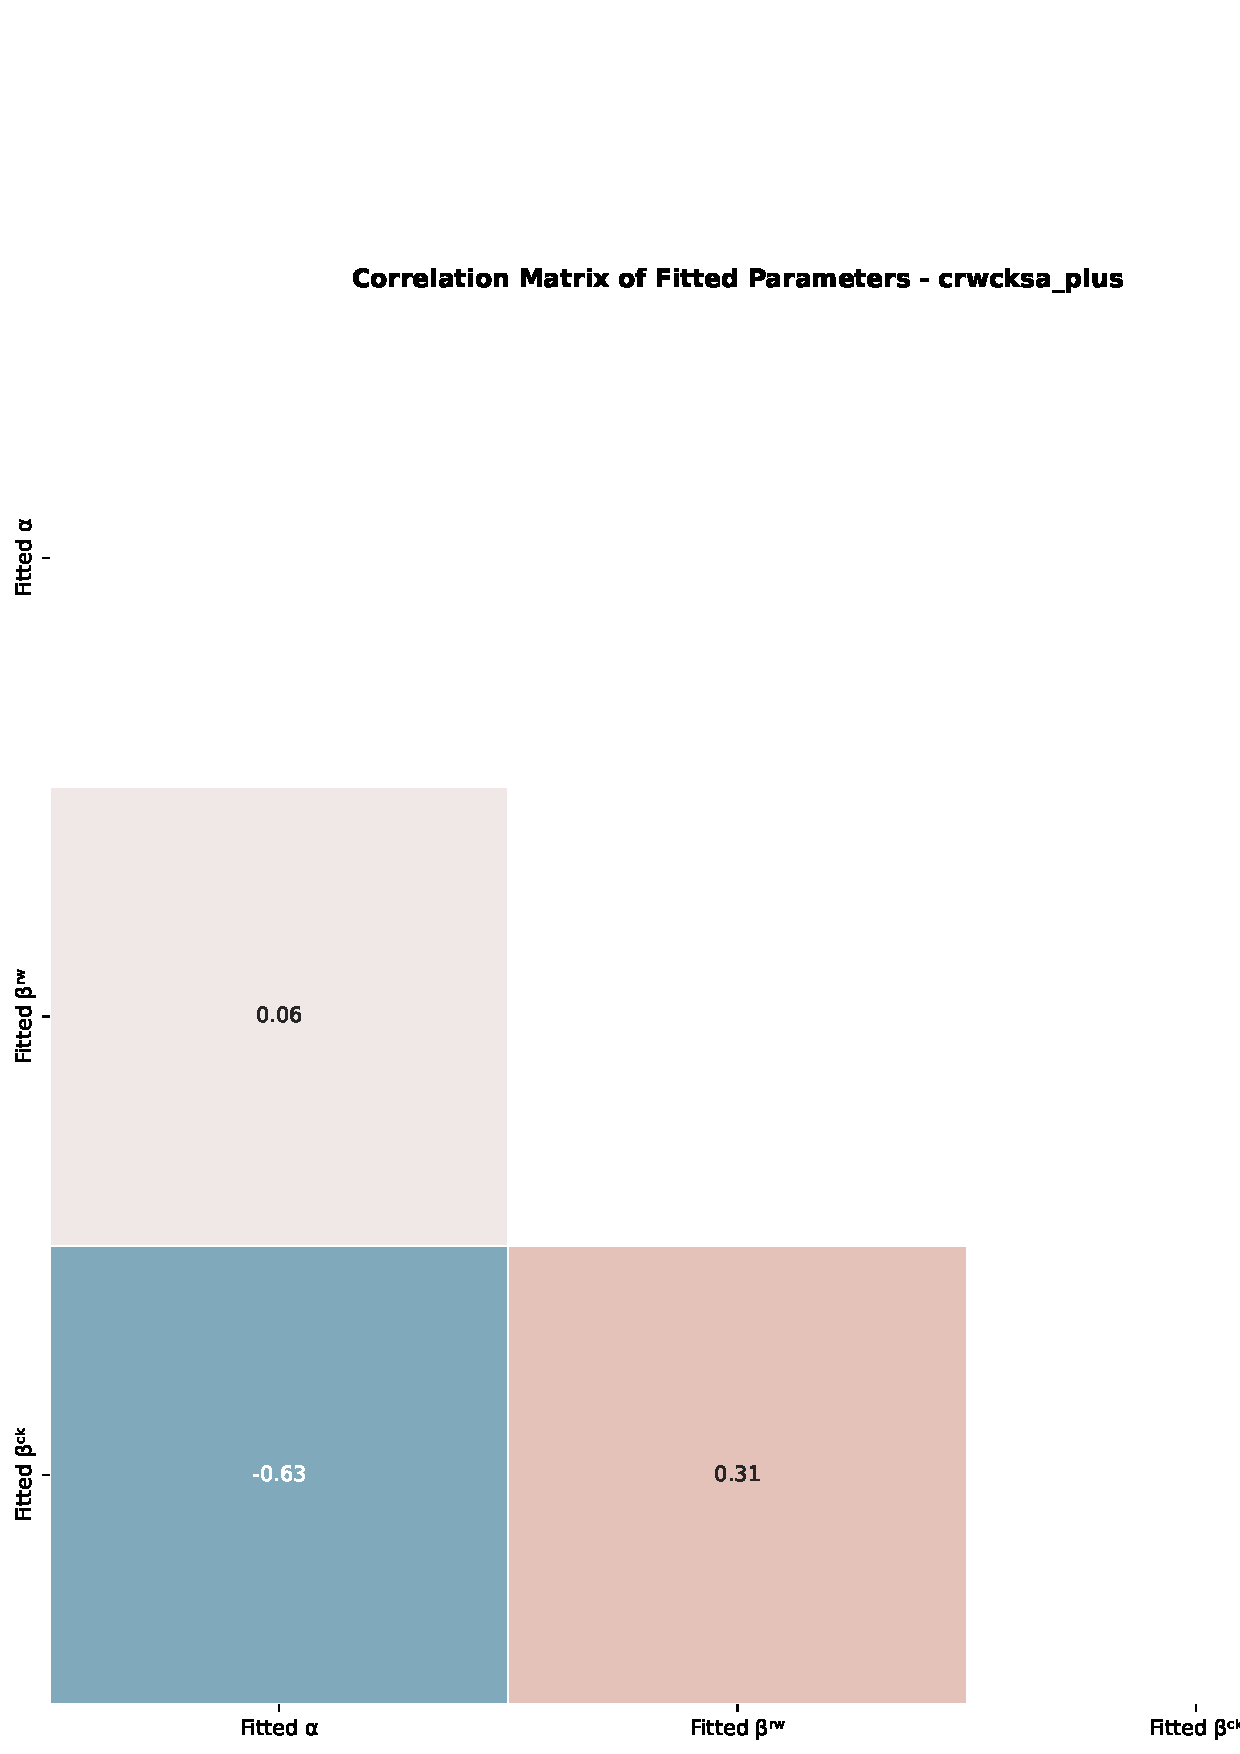
\includegraphics[scale = \correlation]{D:/Documents/Work/Helsinki_Internship/Code/perceptual_attention_learning/reinforcement_learning/plots/correlation/correlation_matrices/crwcksa_plus_correlation.png}  % Change 'image.png' to the name of your image file
	\caption{Correlation matrix of the optimal parameters for the Contextual Rescorla-Wagner Choice-Kernel Shared Alpha Plus model.}
	\label{fig:crwcksa_plus_correlation_matrix}
\end{figure} 

\newpage

\subsection{Contextual Rescorla-Wagner Choice-Kernel Plus Pre-Fitted Parameter Comparison}

\begin{figure}[h]  % [h] places the figure here
	\centering
	\includegraphics[scale = \parameter]{D:/Documents/Work/Helsinki_Internship/Code/perceptual_attention_learning/reinforcement_learning/plots/param_comparison/crwck_plus_pre_param_comparison.png}  % Change 'image.png' to the name of your image file
	\caption{Barchart comparing the optimal parameters for the Contextual Rescorla-Wagner Choice-Kernel Plus Pre-Fitted model.}
	\label{fig:crwck_plus_pre_model_parmeters}
\end{figure} 

\subsubsection{Contextual Rescorla-Wagner Choice-Kernel Plus Pre-Fitted Parameter Correlation Matrix}
\begin{figure}[h]  % [h] places the figure here
	\centering
	\includegraphics[scale = \correlation]{D:/Documents/Work/Helsinki_Internship/Code/perceptual_attention_learning/reinforcement_learning/plots/correlation/correlation_matrices/crwck_plus_pre_correlation.png}  % Change 'image.png' to the name of your image file
	\caption{Correlation matrix of the optimal parameters for the Contextual Rescorla-Wagner Choice-Kernel Plus Pre-Fitted model.}
	\label{fig:crwck_plus_pre_correlation_matrix}
\end{figure} 
\clearpage

\subsection{Contextual Rescorla-Wagner Choice-Kernel Plus Initialised Parameter Comparison}

\begin{figure}[h]  % [h] places the figure here
	\centering
	\includegraphics[scale=\parameter]{D:/Documents/Work/Helsinki_Internship/Code/perceptual_attention_learning/reinforcement_learning/plots/param_comparison/crwck_plus_param_comparison.png}  % Change 'image.png' to the name of your image file
	\caption{Barchart comparing the optimal parameters for the Contextual Rescorla-Wagner Choice-Kernel Plus Initialised model.}
	\label{fig:crwck_plus_init_model_parmeters}
\end{figure} 
\newpage

\section{Order Effects}

\begin{figure}[h]  % [h] places the figure here
	\centering
	\includegraphics[scale=\scale]{D:/Documents/Work/Helsinki_Internship/Code/perceptual_attention_learning/reinforcement_learning/plots/order_effects_comp_first/rr_param_comparison.png}  % Change 'image.png' to the name of your image file
	\caption{Barchart comparing fitted parameters between individuals who did the Easy task first and the Hard task first for the Random Response Model.}
	\label{fig:rr_model_effects}
\end{figure} 

\begin{figure}[h]  % [h] places the figure here
	\centering
	\includegraphics[scale=\scale]{D:/Documents/Work/Helsinki_Internship/Code/perceptual_attention_learning/reinforcement_learning/plots/order_effects_comp_first/crr_param_comparison.png}  % Change 'image.png' to the name of your image file
	\caption{Barchart comparing fitted parameters between individuals who did the Easy task first and the Hard task first for the Contextual Random Response Model.}
	\label{fig:crr_model_effects}
\end{figure} 

\begin{figure}[h]  % [h] places the figure here
	\centering
	\includegraphics[scale=\scale]{D:/Documents/Work/Helsinki_Internship/Code/perceptual_attention_learning/reinforcement_learning/plots/order_effects_comp_first/wsls_param_comparison.png}  % Change 'image.png' to the name of your image file
	\caption{Barchart comparing fitted parameters between individuals who did the Easy task first and the Hard task first for the Win-Stay, Lose-Shift Model.}
	\label{fig:wsls_model_effects}
\end{figure} 

\begin{figure}[h]  % [h] places the figure here
	\centering
	\includegraphics[scale=\scale]{D:/Documents/Work/Helsinki_Internship/Code/perceptual_attention_learning/reinforcement_learning/plots/order_effects_comp_first/rw_param_comparison.png}  % Change 'image.png' to the name of your image file
	\caption{Barchart comparing fitted parameters between individuals who did the Easy task first and the Hard task first for the Rescorla-Wagner Model.}
	\label{fig:rw_model_effects}
\end{figure} 

\begin{figure}[h]  % [h] places the figure here
	\centering
	\includegraphics[scale=\scale]{D:/Documents/Work/Helsinki_Internship/Code/perceptual_attention_learning/reinforcement_learning/plots/order_effects_comp_first/crw_param_comparison.png}  % Change 'image.png' to the name of your image file
	\caption{Barchart comparing fitted parameters between individuals who did the Easy task first and the Hard task first for the Contextual Rescorla-Wagner Model.}
	\label{fig:crw_model_effects}
\end{figure} 

\begin{figure}[h]  % [h] places the figure here
	\centering
	\includegraphics[scale=\scale]{D:/Documents/Work/Helsinki_Internship/Code/perceptual_attention_learning/reinforcement_learning/plots/order_effects_comp_first/ck_param_comparison.png}  % Change 'image.png' to the name of your image file
	\caption{Barchart comparing fitted parameters between individuals who did the Easy task first and the Hard task first for the Contextual Choice-Kernel Model.}
	\label{fig:ck_model_effects}
\end{figure} 

\begin{figure}[h]  % [h] places the figure here
	\centering
	\includegraphics[scale=\scale]{D:/Documents/Work/Helsinki_Internship/Code/perceptual_attention_learning/reinforcement_learning/plots/order_effects_comp_first/crwck_param_comparison.png}  % Change 'image.png' to the name of your image file
	\caption{Barchart comparing fitted parameters between individuals who did the Easy task first and the Hard task first for the Contextual Rescorla-Wagner Choice-Kernel Model.}
	\label{fig:crwck_model_effects}
\end{figure} 

\begin{figure}[h]  % [h] places the figure here
	\centering
	\includegraphics[scale=\scale]{D:/Documents/Work/Helsinki_Internship/Code/perceptual_attention_learning/reinforcement_learning/plots/order_effects_comp_first/crwcksa_param_comparison.png}  % Change 'image.png' to the name of your image file
	\caption{Barchart comparing fitted parameters between individuals who did the Easy task first and the Hard task first for the Contextual Rescorla-Wagner Choice-Kernel Shared Alpha Model.}
	\label{fig:crwcksa_model_effects}
\end{figure} 

\begin{figure}[h]  % [h] places the figure here
	\centering
	\includegraphics[scale=\scale]{D:/Documents/Work/Helsinki_Internship/Code/perceptual_attention_learning/reinforcement_learning/plots/order_effects_comp_first/crwcknb_param_comparison.png}  % Change 'image.png' to the name of your image file
	\caption{Barchart comparing fitted parameters between individuals who did the Easy task first and the Hard task first for the Contextual Rescorla-Wagner Choice-Kernel No Beta Model.}
	\label{fig:crwcknb_model_effects}
\end{figure} 

\begin{figure}[h]  % [h] places the figure here
	\centering
	\includegraphics[scale=\scale]{D:/Documents/Work/Helsinki_Internship/Code/perceptual_attention_learning/reinforcement_learning/plots/order_effects_comp_first/crwck_all_param_comparison.png}  % Change 'image.png' to the name of your image file
	\caption{Barchart comparing fitted parameters between individuals who did the Easy task first and the Hard task first for the Contextual Rescorla-Wagner Choice-Kernel All Model.}
	\label{fig:crwck_all_model_effects}
\end{figure} 

\begin{figure}[h]  % [h] places the figure here
	\centering
	\includegraphics[scale=\scale]{D:/Documents/Work/Helsinki_Internship/Code/perceptual_attention_learning/reinforcement_learning/plots/order_effects_comp_first/crwck_pre_param_comparison.png}  % Change 'image.png' to the name of your image file
	\caption{Barchart comparing fitted parameters between individuals who did the Easy task first and the Hard task first for the Contextual Rescorla-Wagner Choice-Kernel Pre-Fitted Model.}
	\label{fig:crwck_pre_model_effects}
\end{figure} 


\begin{figure}[h]  % [h] places the figure here
	\centering
	\includegraphics[scale=\scale]{D:/Documents/Work/Helsinki_Internship/Code/perceptual_attention_learning/reinforcement_learning/plots/order_effects_comp_first/crwck_init_param_comparison.png}  % Change 'image.png' to the name of your image file
	\caption{Barchart comparing fitted parameters between individuals who did the Easy task first and the Hard task first for the Contextual Rescorla-Wagner Choice-Kernel Initialised Model.}
	\label{fig:crwck_init_model_effects}
\end{figure} 

\begin{figure}[h]  % [h] places the figure here
	\centering
	\includegraphics[scale=\scale]{D:/Documents/Work/Helsinki_Internship/Code/perceptual_attention_learning/reinforcement_learning/plots/order_effects_comp_first/crwck_plus_param_comparison.png}  % Change 'image.png' to the name of your image file
	\caption{Barchart comparing fitted parameters between individuals who did the Easy task first and the Hard task first for the Contextual Rescorla-Wagner Choice-Kernel Plus Model.}
	\label{fig:crwck_plus_model_effects}
\end{figure} 

\begin{figure}[h]  % [h] places the figure here
	\centering
	\includegraphics[scale=\scale]{D:/Documents/Work/Helsinki_Internship/Code/perceptual_attention_learning/reinforcement_learning/plots/order_effects_comp_first/crwcksa_plus_param_comparison.png}  % Change 'image.png' to the name of your image file
	\caption{Barchart comparing fitted parameters between individuals who did the Easy task first and the Hard task first for the Contextual Rescorla-Wagner Choice-Kernel Shared Alpha Plus Model.}
	\label{fig:crwcksa_plus_model_effects}
\end{figure} 

\begin{figure}[h]  % [h] places the figure here
	\centering
	\includegraphics[scale=\scale]{D:/Documents/Work/Helsinki_Internship/Code/perceptual_attention_learning/reinforcement_learning/plots/order_effects_comp_first/crwck_plus_pre_param_comparison.png}  % Change 'image.png' to the name of your image file
	\caption{Barchart comparing fitted parameters between individuals who did the Easy task first and the Hard task first for the Contextual Rescorla-Wagner Choice-Kernel Plus Pre-Fitted Model.}
	\label{fig:crwck_plus_pre_model_effects}
\end{figure} 

\begin{figure}[h]  % [h] places the figure here
	\centering
	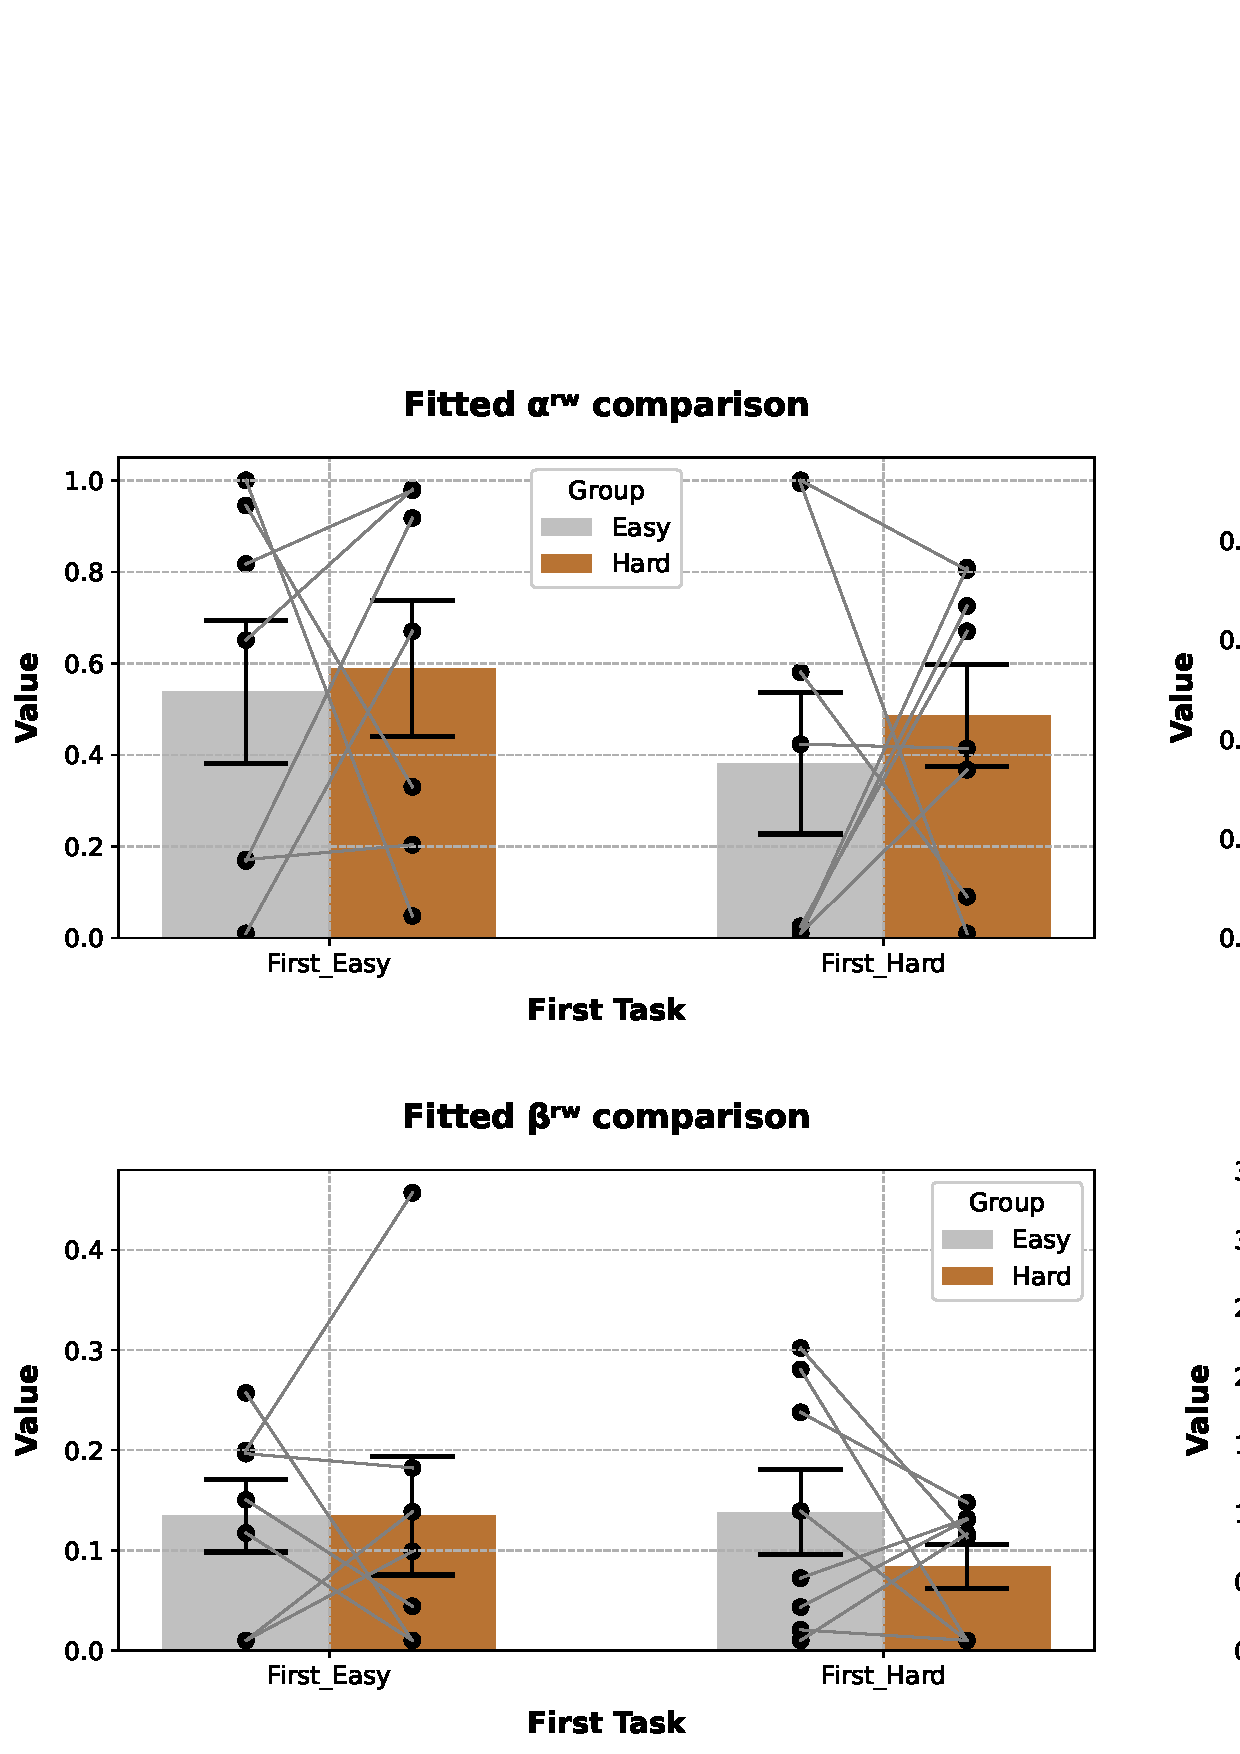
\includegraphics[scale=\scale]{D:/Documents/Work/Helsinki_Internship/Code/perceptual_attention_learning/reinforcement_learning/plots/order_effects_comp_first/crwck_plus_init_param_comparison.png}  % Change 'image.png' to the name of your image file
	\caption{Barchart comparing fitted parameters between individuals who did the Easy task first and the Hard task first for the Contextual Rescorla-Wagner Choice-Kernel Plus Initialised Model.}
	\label{fig:crwck_plus_init_model_effects}
\end{figure} 

\clearpage

\section{Model Prediction versus Reality}
In the last 100 trials, the estimated GO probability was calculated for best fitting model (crwcksa\_plus) and was overlaid with the actual actions of rat subjects as well as the stimuli received. We present some of these plots below.

\begin{figure}[h]  % [h] places the figure here
	\centering
	\includegraphics[scale=\scaletwo]{D:/Documents/Work/Helsinki_Internship/Code/perceptual_attention_learning/reinforcement_learning/plots/sim_vs_reality/crwcksa_plus/crwcksa_plus_Easy_422.0_last_sim_vs_reality.png}  % Change 'image.png' to the name of your image file
	\caption{Line graph comparing the predicted GO probability and action taken for rat subject 422's last 100 trials during the Easy EDS}
	\label{fig:422_easy}
\end{figure} 

\begin{figure}[h]  % [h] places the figure here
	\centering
	\includegraphics[scale=\scaletwo]{D:/Documents/Work/Helsinki_Internship/Code/perceptual_attention_learning/reinforcement_learning/plots/sim_vs_reality/crwcksa_plus/crwcksa_plus_Hard_422.0_last_sim_vs_reality.png}  % Change 'image.png' to the name of your image file
	\caption{Line graph comparing the predicted GO probability and action taken for rat subject 422's last 100 trials during the Hard EDS}
	\label{fig:422_hard}
\end{figure} 

\begin{figure}[h]  % [h] places the figure here
	\centering
	\includegraphics[scale=\scaletwo]{D:/Documents/Work/Helsinki_Internship/Code/perceptual_attention_learning/reinforcement_learning/plots/sim_vs_reality/crwcksa_plus/crwcksa_plus_Easy_4151.0_last_sim_vs_reality.png}  % Change 'image.png' to the name of your image file
	\caption{Line graph comparing the predicted GO probability and action taken for rat subject 4151's last 100 trials during the Easy EDS}
	\label{fig:4151_easy}
\end{figure} 

\begin{figure}[h]  % [h] places the figure here
	\centering
	\includegraphics[scale=\scaletwo]{D:/Documents/Work/Helsinki_Internship/Code/perceptual_attention_learning/reinforcement_learning/plots/sim_vs_reality/crwcksa_plus/crwcksa_plus_Hard_4151.0_last_sim_vs_reality.png}  % Change 'image.png' to the name of your image file
	\caption{Line graph comparing the predicted GO probability and action taken for rat subject 4151's last 100 trials during the Hard EDS}
	\label{fig:4151_hard}
\end{figure} 
\begin{figure}[h]  % [h] places the figure here
	\centering
	\includegraphics[scale=\scaletwo]{D:/Documents/Work/Helsinki_Internship/Code/perceptual_attention_learning/reinforcement_learning/plots/sim_vs_reality/crwcksa_plus/crwcksa_plus_Easy_5091.0_last_sim_vs_reality.png}  % Change 'image.png' to the name of your image file
	\caption{Line graph comparing the predicted GO probability and action taken for rat subject 5091's last 100 trials during the Easy EDS}
	\label{fig:5091_easy}
\end{figure} 

\begin{figure}[h]  % [h] places the figure here
	\centering
	\includegraphics[scale=\scaletwo]{D:/Documents/Work/Helsinki_Internship/Code/perceptual_attention_learning/reinforcement_learning/plots/sim_vs_reality/crwcksa_plus/crwcksa_plus_Hard_5091.0_last_sim_vs_reality.png}  % Change 'image.png' to the name of your image file
	\caption{Line graph comparing the predicted GO probability and action taken for rat subject 5091's last 100 trials during the Hard EDS}
	\label{fig:5091_hard}
\end{figure} 
\clearpage

\section{Discussion}

Correlation matrices were plotted for the more complex model to see if there was redundancy in the fitted parameters, possibly indicating over-fitting. There was significant correlation found between parameters for the crwck and crwck\_plus models, hence three new models were fitted, namely the crwcknb, crwcksa and crwcksa\_plus models in order to test whether certain parameters were indeed redundant. The crwcknb model did not perform well relative to other models, indicating that including the Beta/Randomness parameter was in fact useful and necessary. The crwcksa and crwcksa\_plus models performed very similarly to their counterpart models of crwck and crwck\_plus respectively, and based on BIC scores, the crwcka\_plus model in fact came out as the most parsimonious yet expressive model.
\\\\
By the comparison of the parameters of the crwcksa\_plus model in \ref{fig:crwcksa_plus_model_parmeters} we see that on average, the fitted learning rate was higher for the Hard to distinguish group than the easy to distinguish group. Both groups placed more weighting on their Q values than their CK-values in their decision making, as shown by the higher values of $\beta_{ck}$ as compared to $\beta_{rw}$. The Hard to distinguish group applied more randomness in it's decisions on average, as shown by the smaller fitted $\beta_{rw}$ and $\beta_{ck}$ values.
\\\\
In terms of the order effects, in plot \ref{fig:crwcksa_plus_model_effects} we see individuals who were exposed the Easy EDS session first had higher average learning rates across both EDS and Hard sessions as compared to the individuals who were first exposed to the Hard EDS session.
\\\\
Interestingly, initialisation of Q and CK-values using pre-EDS sessions did not improve the fit of the models.
\newpage
\clearpage

\printbibliography[title={References}, heading=bibintoc] % Prints bibliography with numbers

\end{document}



\begin{align}
	CK^i_0 &= \begin{cases}
		CK^i_0 + \alpha_{\text{ck}}\left(1 - CK^i_0 \right)  \qquad \text{if } a_t = 0\\
		CK^i_0 + \alpha_{\text{ck}}\left(0 - CK^i_0 \right)  \qquad \text{if } a_t = 1
	\end{cases}\\
	CK^i_1 &= \begin{cases}
		CK^i_1 + \alpha_{\text{ck}}\left(0 - CK^i_1 \right)  \qquad \text{if } a_t = 0\\
		CK^i_1 + \alpha_{\text{ck}}\left(1 - CK^i_1 \right)  \qquad \text{if } a_t = 1
	\end{cases}.
\end{align}
